\section{Computation architectures}
\label{sec:comparch}
\todo{savner en form for indledning MP}
Computations are often performed on a computer's  \acrshort{cpu}.
A \acrshort{cpu} is often fastest for calculations and task not requiring immense computing power, as well as any calculation not parallelisable.
The \acrshort{cpu} consists of only a few cores which are very fast at performing sequential serial processing.\citep{whatisgpu}
In recent years developers and scientists seem to have developed an interest for performing calculations on Dedicated Graphic Processing Units. \citep{gpurise}\todo{Dette er eneste gang vi benytter dette udtryk, ændres til GPU? MP}
This is a different architecture which was intended for graphics processing.
It seems that the \acrshort{gpu} can be utilised for General-Purpose computing for some computational problems, with a performance improvement over a \acrshort{cpu}.
In the following text we explore the possibilities that a \acrshort{gpu} architecture offers.
\todo{Vi har lige skrevet det her i indledningen ? Skal det med igen ? Eller slet ? - Søren}

\acrshort{gpu}s are commonly used in both private and professional environments, for games and accelerating graphic intensive programs such as Adobe Photoshop and 3D rendering tools.\citep{NVIDIAADOBE,STEAMHW}
The \acrshort{gpu} architecture can also be used advantageously for certain types of computations, primarily computations which can be done in parallel. 
An example of this can be calculating different properties of the pixels on a screen. 
The screen can then be divided into different sections called blocks and the computations for each block of data is divided internally on the \acrshort{gpu} to its threads.
This is possible because the specific calculations do not require results from the other calculations, i.e. they are parallelisable.
Unlike the cores in the \acrshort{cpu}; the cores in the \acrshort{gpu} are not designed to perform sequential serial processing, instead its cores are designed to handle multiple tasks at once. 
As such running sequential code on the \acrshort{cpu} will run faster, whereas more compute-intensive functions may be better suited for the \acrshort{gpu}, given the computations can be parallelised.\citep{NvidiaGPGPU}
The aforementioned example with pixels can be viewed as a matrix being divided into blocks, so the same method of parallelised workflow can be applied. 
For linear algebra, there are especially many operations on matrices where the problem can be split to independent subproblems.

\begin{figure}[h!]
\centering
 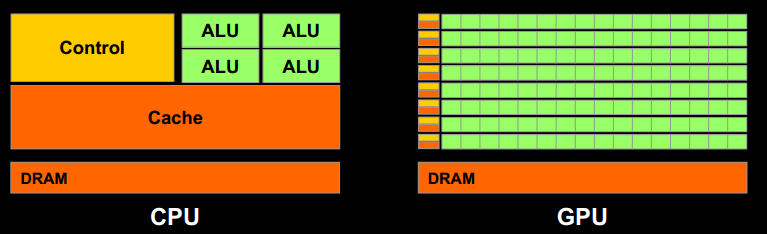
\includegraphics[width=1\textwidth]{figures/GPUCPUimage.png} % trim=4.85cm 15cm 0.85cm 1cm
\caption{A basic representation of the Transistor allocation on a \acrshort{gpu} compared to a \acrshort{cpu}.\citep{NvidiaCUDASeminar}}\label{image:gpucpuimage}
\vspace{-15pt}
\end{figure}

A simple representational comparison of a \acrshort{cpu}'s --- and a \acrshort{gpu}'s transistor usage is shown in \myref{image:gpucpuimage}.
The \acrshort{gpu} consists of many less powerful cores where the \acrshort{cpu} consists of a few more powerful ones, the greater amount of cores allows for more computational power.
But to be able to utilise this computation power a problem must able to be split up, so many or all the cores in the \acrshort{gpu} is used.
As of Q1 2015 an example of a modern high end desktop \acrshort{cpu} is the Intel Haswell core i7 5960X which has 8 cores.\citep{puget}
A contemporary high end \acrshort{gpu} is the NVIDIA GTX 980 which has 2048 CUDA cores.\citep{techpowerup,gtx980}
Due to their architectural differences the \acrshort{gpu} allows for about 12 times more operations per second.\todo{Vi kan sætte en fodnote ind med de beregninger der var her tidligere evt :P ? - Søren}

This makes the \acrshort{gpu} particularly useful for large and complex computations if it is\todo{when it is, måske MP} possible to distribute the workload among the \acrshort{gpu}'s cores.
However, the \acrshort{gpu} has an overhead cost.
This means that moving data and computations to the \acrshort{gpu} is time consuming.
Therefore the computation must be of a certain size, before the advantage of parallel \acrshort{gpu} computations exceeds the cost of transferring calculations onto the \acrshort{gpu}.
To illustrate this problem as well as finding an approximate computation size where the \acrshort{gpu} is advantageous some test problems have been written. 
These problems perform different operations on all elements in a matrix. 

\subsection{\acrshort{gpu} and \acrshort{cpu} computations comparison}\label{sub:gpubenchmark}
To compare the computational speed of a \acrshort{gpu} and a \acrshort{cpu} for operations on each element in a matrix we have written two programs.
A program written in regular C targeting the \acrshort{cpu} and an equivalent program written in C with CUDA libraries targeting the \acrshort{gpu} for computations.
\todo{Skal der ikke stå noget om hvad CUDA er her ?}
Further explanation of this test and the full source code of both programs and the accompanying scripts can be found in \myref{app:gpuoverhead} and \myref{app:cd}.

Both programs have been run with multiple sizes of the matrix.
The execution times for the two have been compared to find an estimated threshold for when the \acrshort{gpu} power\todo{Andet ydtryk end power, performance? MP} overtakes the data transfer.
The test case for the following comparison consists of seven operations on a square matrix of size n.
As an example, with a square matrix of size $n$ as input the amount of calculations is $7*n^2 = O(n^2)$ operations. 
And there are $n^2 = O(n^2)$ numbers in the matrix which will be operated on.\todo{Matrix entries/elements MP}
The operations are division, multiplication, addition and subtraction.
The result can be seen on \myref{image:benchmark}.
\begin{figure}[h!]
\centering
 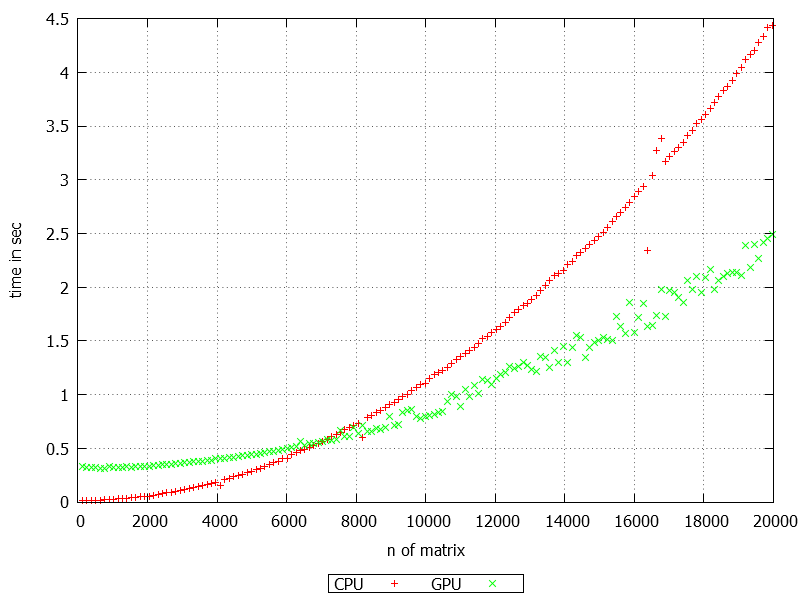
\includegraphics[width=1\textwidth]{figures/benchmark.png} % trim=4.85cm 15cm 0.85cm 1cm
\caption{A benchmark of performing seven operations on each element in a square matrix with size n on a \acrshort{cpu} and a \acrshort{gpu} respectively.}\label{image:benchmark}
\vspace{-15pt}
\end{figure}

The results show that in this case the \acrshort{gpu} becomes advantageous when n reaches about 7000 as can be seen in \myref{image:benchmark}
When n is 7000 the size of the matrix represent operations on almost 50 millions elements.
This is a large amount of data but this is partly due to the simple operations done on the elements in the matrix, we believe that the threshold would happen earlier for more complex operations on the elements in matrix.\todo{og hvorfra ved vi at det er fordi det er simple operationer? og hvorfor mener vi thresholden ændres med andre operationer?}
In addition to the threshold, the result also confirms that as the dataset grows the \acrshort{gpu} becomes exponentially more useful for computing the data fast.
